\hypertarget{turtles-manual}{%
\section{Turtle's manual}\label{turtles-manual}}

Turtle is a simple interpreter for turtle graphics.

\hypertarget{prerequisite-and-compiling}{%
\subsection{Prerequisite and
compiling}\label{prerequisite-and-compiling}}

Turtle is written in C language. You need:

\begin{itemize}
\tightlist
\item
  Linux. Turtle is tested on ubuntu 20.10
\item
  gcc, meson and ninja
\item
  gtk4
\end{itemize}

It is easy to compile the source file of turtle. If you have installed
gtk4 with an option \passthrough{\lstinline!--prefix=$HOME/local!}, put
the same option to meson so that you can install
\passthrough{\lstinline!turtle!} under the directory
\passthrough{\lstinline!$HOME/local/bin!}. The instruction is:

\begin{lstlisting}
$ meson --prefix=$HOME/local _build
$ ninja -C _build
$ ninja -C _build install
\end{lstlisting}

Type the following command then turtle shows the following window.

\begin{lstlisting}
$ turtle
\end{lstlisting}

\begin{figure}
\centering
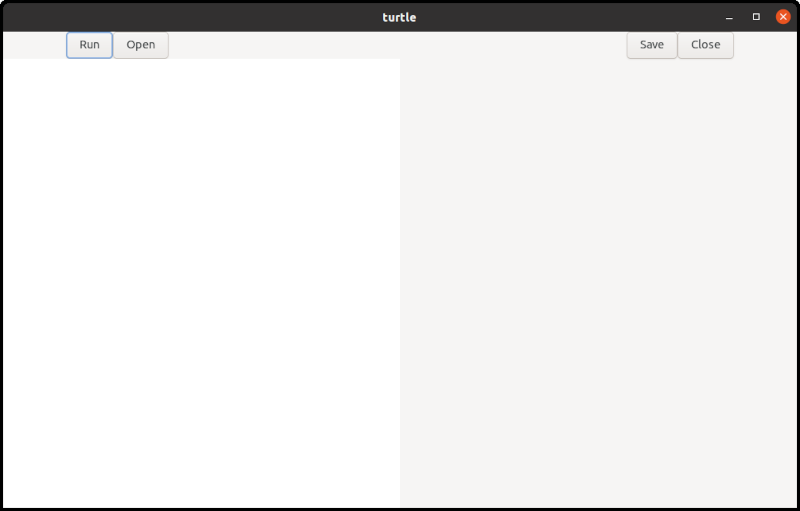
\includegraphics[width=8cm,height=5.11cm]{../src/turtle/image/turtle1.png}
\caption{Screenshot just after it's executed}
\end{figure}

The left half is a text editor and the right half is a surface. Surface
is like a canvas to draw shapes.

Write turtle language in the text editor and click on
\passthrough{\lstinline!run!} button, then the program will be executed
and it draws shapes on the surface.

\begin{figure}
\centering
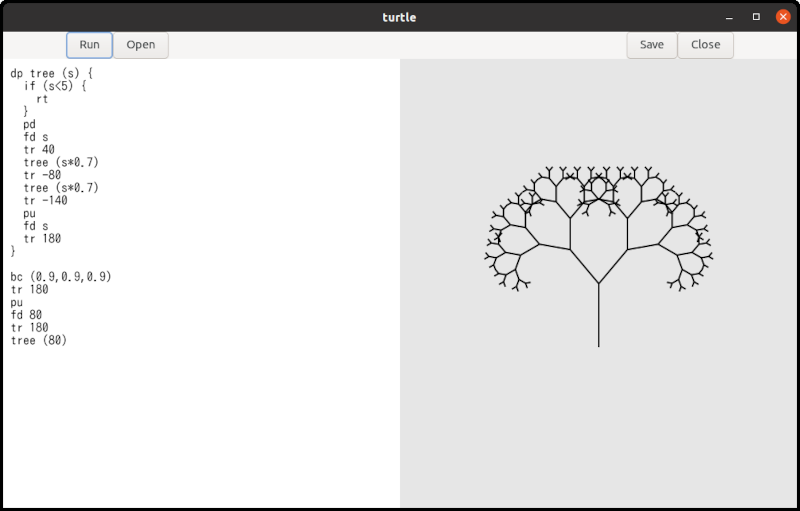
\includegraphics[width=8cm,height=5.11cm]{../src/turtle/image/turtle_tree.png}
\caption{Tree}
\end{figure}

If you add the following line in \passthrough{\lstinline!turtle.h!},
then codes to inform the status will also be compiled. However, the
speed will be quite slow because of the output messages.

\begin{lstlisting}
# define debug 1
\end{lstlisting}

\hypertarget{example}{%
\subsection{Example}\label{example}}

Imagine a turtle. The turtle has a pen and initially he is at the center
of the screen, facing to the north (to the north means up on the
screen). You can let the turtle down the pen or up the pen. You can
order the turtle to move forward.

\begin{lstlisting}
pd
fd 100
\end{lstlisting}

\begin{itemize}
\tightlist
\item
  pd: Pen Down. The turtle put the pen down so that the turtle will draw
  a line if he/she moves.
\item
  fd 100: move ForwarD 100. The turtle goes forward 100 pixels.
\end{itemize}

If you click on \passthrough{\lstinline!run!} button, then a line
segment appears on the screen. One of the endpoints of the line segment
is at the center of the surface and the other is at 100 pixels up from
the center. The point at the center is the start point of the turtle and
the other endpoint is the end point of the movement.

If the turtle picks the pen up, then no line segment appears.

\begin{lstlisting}
pu
fd 100
\end{lstlisting}

The command \passthrough{\lstinline!pu!} means ``Pen Up''.

The turtle can change the direction.

\begin{lstlisting}
pd
fd 100
tr 90
fd 100
\end{lstlisting}

The command \passthrough{\lstinline!tr!} is ``Turn Right''. The argument
is angle with degrees. Therefore, \passthrough{\lstinline!tr 90!} means
``Turn right by 90 degrees''. If you click on the
\passthrough{\lstinline!run!}button, then two line segments appears. One
is vertical and the other is horizontal.

\begin{figure}
\centering
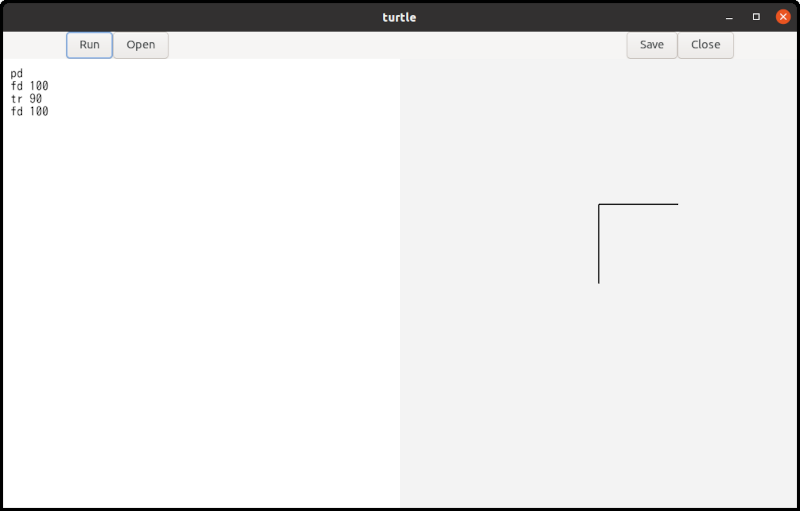
\includegraphics[width=8cm,height=5.11cm]{../src/turtle/image/turtle2.png}
\caption{Two line segments on the surface}
\end{figure}

\hypertarget{background-and-foreground-color}{%
\subsection{Background and foreground
color}\label{background-and-foreground-color}}

Colors are specified with RGB. A vector (r, g, b) denotes RGB color.
Each of the elements is a real number between 0 and 1.

\begin{itemize}
\tightlist
\item
  Red is (1.0, 0.0, 0.0). You can write (1, 0, 0) instead.
\item
  Green is (0.0, 1.0, 0.0)
\item
  Blue is (0.0, 0.0, 1.0)
\item
  Black is (0.0, 0.0, 0.0)
\item
  White is (1.0, 1.0, 1.0)
\end{itemize}

You can express a variety of colors by changing each element.

There are two commands to change colors.

\begin{itemize}
\tightlist
\item
  bc: Background Color. \passthrough{\lstinline!bc (1,0,0)!} changes the
  background color to red. This command clear the surface and change the
  background color. So, the shapes on the surface disappears.
\item
  fc: Foreground Color. \passthrough{\lstinline!fc (0,1,0)!} changes the
  foreground color to green. This command changes the pen color. The
  prior shapes on the surface aren't affected. After this command, the
  turtle draws lines with the new color.
\end{itemize}

\begin{figure}
\centering
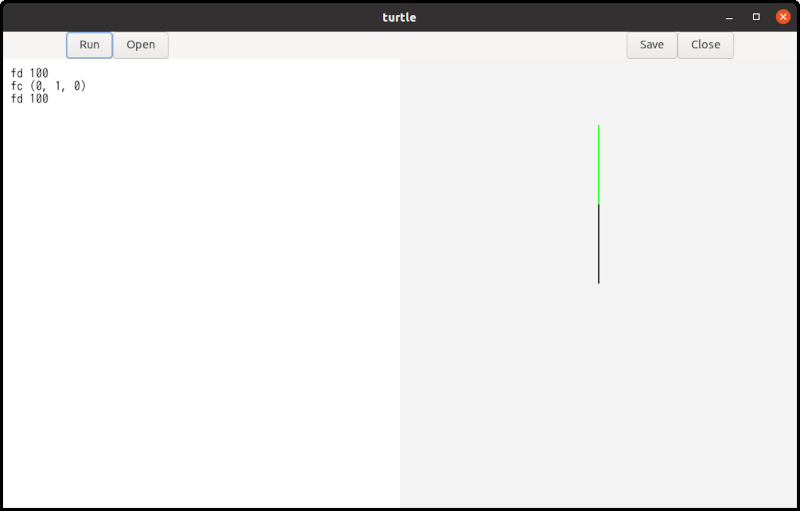
\includegraphics[width=8cm,height=5.11cm]{../src/turtle/image/turtle3.png}
\caption{Change the foreground color}
\end{figure}

\hypertarget{other-simple-commands}{%
\subsection{Other simple commands}\label{other-simple-commands}}

\begin{itemize}
\tightlist
\item
  pw: Pen Width. This is the same as pen size or line width. For
  example, \passthrough{\lstinline!pw 5!} makes lines thick and
  \passthrough{\lstinline!pw 1!} makes it thin.
\item
  rs: ReSet. The turtle moves back to the initial position and
  direction. In addition, The command initialize the pen, line width
  (pen size), and foreground color. The pen is down, the line width is 2
  and the foreground color is black.
\end{itemize}

An order such as \passthrough{\lstinline!fd 100!},
\passthrough{\lstinline!pd!} and so on is a statement. Statements are
executed in the order from the top to the end

\hypertarget{comment-and-spaces}{%
\subsection{Comment and spaces}\label{comment-and-spaces}}

Characters between \passthrough{\lstinline!\#!} (hash mark) and
\passthrough{\lstinline!\\n!} (new line) inclusive are comment. If the
comment is at the end of the file, the trailing new line can be left
out. Comments are ignored.

\begin{lstlisting}
# draw a triangle
fd 100 # forward 100 pixels<NEW LINE>
tr 120 # turn right by 90 degrees<NEW LINE>
fd 100<NEW LINE>
tr 120<NEW LINE>
fd 100 # Now a triangle appears.<EOF>
\end{lstlisting}

\textless NEW LINE\textgreater{} and \textless EOF\textgreater{}
indicate newline code and end of file respectively. The comments in the
line 1, 2, 3 and 6 are correct syntactically.

Spaces (white space, tab and new line) are ignored. They are used only
as delimiters. Tabs are recognized as eight spaces to calculate the
column number.

\hypertarget{variables-and-expressions}{%
\subsection{Variables and expressions}\label{variables-and-expressions}}

Variable begins alphabet followed by alphabet or digit. Key words like
\passthrough{\lstinline!fd!}, \passthrough{\lstinline!tr!} can't be
variables. \passthrough{\lstinline!Distance!} and
\passthrough{\lstinline!angle5!} are variables, but
\passthrough{\lstinline!1step!} isn't a variable because the first
character isn't alphabet. Variable names are case sensitive. Variables
keep real numbers. Their type is the same as
\passthrough{\lstinline!double!} in C language. Integers are casted to
real numbers automatically. So 1 and 1.0 are the same value. Numbers
begin digits, not signs (\passthrough{\lstinline!+!} or
\passthrough{\lstinline!-!}).

\begin{itemize}
\tightlist
\item
  100, 20.34 and 0.01 are numbers
\item
  +100 isn't a number. It causes syntax error. Use 100 instead.
\item
  -100 isn't a number. But turtle recognizes it unary minus and a number
  100. So turtle calculate it and the result is -100.
\item
  100 + -20: This is recognized 100 + (- 20). However, using bracket,
  100 + (-20), is better for easy reading.
\end{itemize}

\begin{lstlisting}
distance = 100
fd distance
\end{lstlisting}

A value 100 is assigned to the variable
\passthrough{\lstinline!distance!} in the first line. Assignment is a
statement. Most of statements begin with commands like
\passthrough{\lstinline!fd!}. Assignment is the only exception.

The example above draws a line segment of 100 pixels long.

You can use variables in expressions. There are 8 kinds of calculations
available.

\begin{itemize}
\tightlist
\item
  addition: x + y
\item
  subtraction: x - y
\item
  multiplication: x * y
\item
  division: x / y
\item
  unary minus: - x
\item
  logical equal: x = y. This symbol \passthrough{\lstinline!=!} works as
  \passthrough{\lstinline!==!} in C language.
\item
  greater than: x \textgreater{} y
\item
  less than: x \textless{} y
\end{itemize}

The last three symbols are mainly used in the condition of if statement.

Variables are registered to a symbol table when it is assigned a value
for the first time. Evaluating a variable before the registration isn't
allowed and occurs an error.

\hypertarget{if-statement}{%
\subsection{If statement}\label{if-statement}}

Turtle language has very simple if statement.

\begin{lstlisting}
if (x > 50) {
  fd x
}
\end{lstlisting}

There is no else part.

\hypertarget{procedures}{%
\subsection{Procedures}\label{procedures}}

Procedures are similar to functions in C language. The difference is
that procedures don't have return values.

\begin{lstlisting}
dp triangle (side) {
  fd side
  tr 120
  fd side
  tr 120
  fd side
}

triangle (100)
\end{lstlisting}

\passthrough{\lstinline!dp!} (Define Procedure) is a key word followed
by procedure name, parameters, and body. Procedure names start alphabet
followed by alphabet or digit. Parameters are a list of variables. For
example

\begin{lstlisting}
dp abc (a) { ... ... }
dp abc (a, b) { ... ... }
dp abc (a, b, c) { ... ... }
\end{lstlisting}

Body is a sequence of statements. The statements aren't executed when
the procedure is defined. They will be executed when the procedure is
called later.

Procedures are called by the name followed by arguments.

\begin{lstlisting}
dp proc (a, b, c) { ... ... }

proc (100, 0, -20*3)
\end{lstlisting}

The number of parameters and arguments must be the same. Arguments can
be any expressions. When you call a procedure, brackets following the
procedure name must exist even if the procedure has no argument.

Procedure names and variable names don't conflict.

\begin{lstlisting}
dp a () {fd a}
a=100
a ()
\end{lstlisting}

This is a correct program.

\begin{itemize}
\tightlist
\item
  1: Defines a procedure \passthrough{\lstinline!a!}. A variable
  \passthrough{\lstinline!a!} is in its body.
\item
  2: Assigns 100 to a variable \passthrough{\lstinline!a!}.
\item
  3: Procedure \passthrough{\lstinline!a!} is called.
\end{itemize}

However, using the same name to a procedure and variable makes
confusing. You should avoid that.

\hypertarget{recursive-call}{%
\subsection{Recursive call}\label{recursive-call}}

Procedures can be called recursively.

\begin{lstlisting}
dp repeat (n) {
  n = n - 1
  if (n < 0) {
    rt
  }
  fd 100
  tr 90
  repeat (n)
}

repeat (4)
\end{lstlisting}

Repeat is called in the body of repeat. The call to itself is a
recursive call. Parameters are created and set each time the procedure
is called. So, parameter \passthrough{\lstinline!n!} is 4 at the first
call but it is 3 at the second call. Each time the procedure is called,
the parameter \passthrough{\lstinline!n!} decreases by one. Finally, it
becomes less than zero, then the procedures return.

The program above draws a square.

Turtle doesn't have any primary loop statements. It should probably be
added to the future version. However, the program above shows that we
can program loop with a recursive call.

\hypertarget{fractal-curves}{%
\subsection{Fractal curves}\label{fractal-curves}}

Recursive call can be applied to draw fractal curves. Fractal curves
appear when a procedure is applied to it repeatedly. The procedure
replaces a part of the curve with the contracted curve.

\begin{figure}
\centering
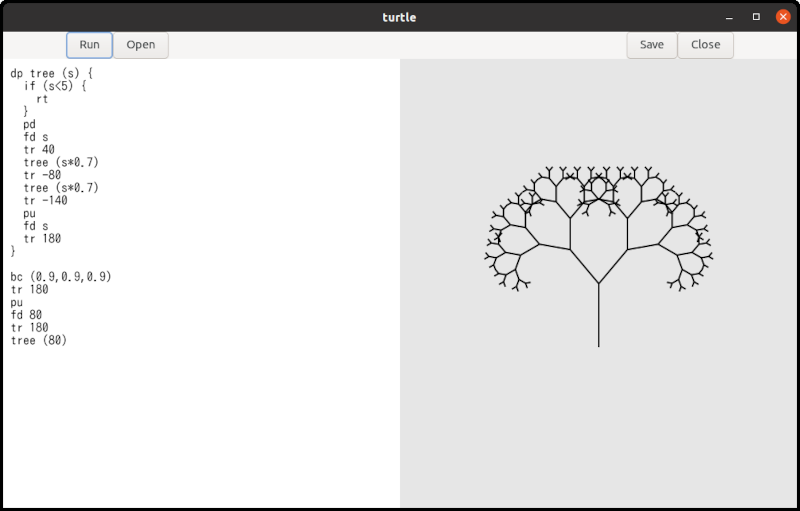
\includegraphics[width=8cm,height=5.11cm]{../src/turtle/image/turtle_tree.png}
\caption{Tree}
\end{figure}

This shape is called tree. The basic pattern of this shape is a line
segment. It is the first stage. The second stage adds two shorter line
segments at the endpoint of the original segment. The new segment has 70
percent length to the original segment and the orientation is +30 or -30
degrees different. The third stage adds two shorter line segments to the
second stage line segments. And repeats it several times.

This repeating is programmed by recursive call. Two more examples are
shown here. They are Koch curve and Square Koch curve.

\begin{figure}
\centering
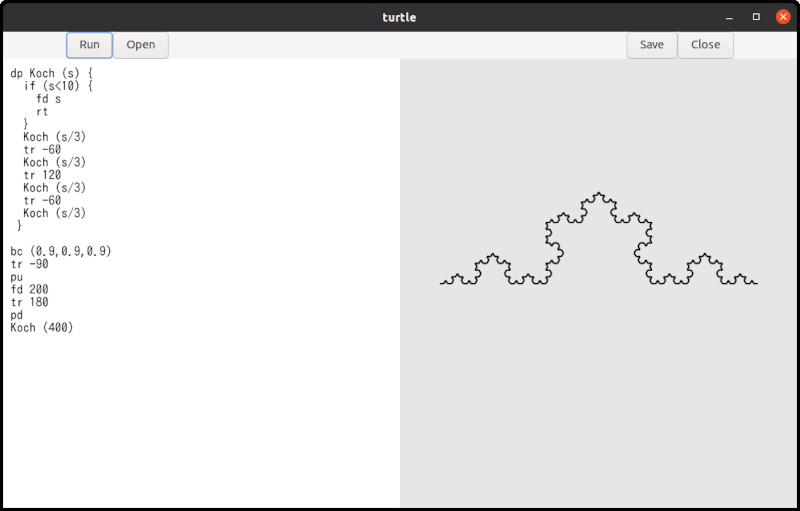
\includegraphics[width=8cm,height=5.11cm]{../src/turtle/image/turtle_koch.png}
\caption{Koch curve}
\end{figure}

\begin{figure}
\centering
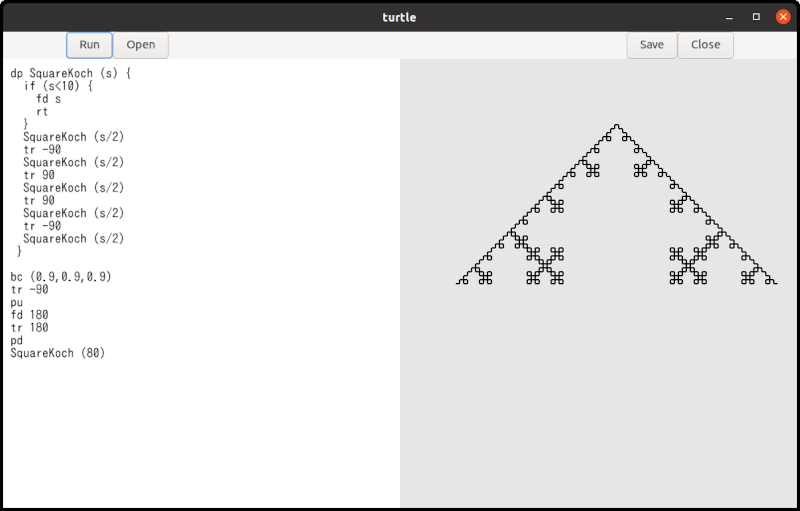
\includegraphics[width=8cm,height=5.11cm]{../src/turtle/image/turtle_square_koch.png}
\caption{Square Koch curve}
\end{figure}

\hypertarget{tokens-and-punctuations}{%
\subsection{Tokens and punctuations}\label{tokens-and-punctuations}}

The following is the list of tokens.

Keywords:

\begin{itemize}
\tightlist
\item
  pu: pen up
\item
  pd: pen down
\item
  pw: pen width = line width
\item
  fd: forward
\item
  tr: turn right
\item
  bc: background color
\item
  fc: foreground color
\item
  if: if statement
\item
  rt: return
\item
  rs: reset
\item
  dp: define procedure
\end{itemize}

identifiers and numbers:

\begin{itemize}
\tightlist
\item
  identifier: This is used for the name of variables, parameters and
  procedures. It is expressed
  \passthrough{\lstinline![a-zA-Z][a-zA-Z0-9]*!} in regular expression.
\item
  number: This is expressed
  \passthrough{\lstinline!(0|[1-9][0-9]*)(\\.[0-9]+)?!} in regular
  expression. It doesn't have \passthrough{\lstinline!+!} or
  \passthrough{\lstinline!-!} sign because they bring some syntactic
  confusion. However negative number such as
  \passthrough{\lstinline!-10!} can be recognized as unary minus and a
  number.
\end{itemize}

Symbols for expression

\begin{itemize}
\tightlist
\item
  \passthrough{\lstinline!=!}
\item
  \passthrough{\lstinline!>!}
\item
  \passthrough{\lstinline!<!}
\item
  \passthrough{\lstinline!+!}
\item
  \passthrough{\lstinline!-!}
\item
  \passthrough{\lstinline!*!}
\item
  \passthrough{\lstinline!/!}
\item
  \passthrough{\lstinline!(!}
\item
  \passthrough{\lstinline!)!}
\end{itemize}

Delimiters

\begin{itemize}
\tightlist
\item
  \passthrough{\lstinline!(!}
\item
  \passthrough{\lstinline!)!}
\item
  \passthrough{\lstinline!\{!}
\item
  \passthrough{\lstinline!\}!}
\item
  \passthrough{\lstinline!,!}
\end{itemize}

Comments and spaces:

\begin{itemize}
\tightlist
\item
  comment: This is characters between \passthrough{\lstinline!\#!} and
  new line inclusive. If a comment is at the end of the file, the
  trailing new line can be left out.
\item
  white space:
\item
  horizontal tab: tab is recognized as eight spaces.
\item
  new line: This is the end of a line.
\end{itemize}

These characters are used to separate tokens explicitly. They doesn't
have any syntactic meaning and are ignored by the parser.

\hypertarget{grammar}{%
\subsection{Grammar}\label{grammar}}

\begin{lstlisting}
program:
  statement
| program statement
;

statement:
  primary_procedure
| procedure_definition
;

primary_procedure:
  PU
| PD
| PW expression
| FD expression
| TR expression
| BC '(' expression ',' expression ',' expression ')'
| FC '(' expression ',' expression ',' expression ')'
| ID '=' expression
| IF '(' expression ')' '{' primary_procedure_list '}'
| RT
| RS
| ID '(' ')'
| ID '(' argument_list ')'
;

procedure_definition:
  DP ID '('  ')' '{' primary_procedure_list '}'
| DP ID '(' parameter_list ')' '{' primary_procedure_list '}'
;

parameter_list:
  ID
| parameter_list ',' ID
;

argument_list:
  expression
| argument_list ',' expression
;

primary_procedure_list:
  primary_procedure
| primary_procedure_list primary_procedure
;

expression:
  expression '=' expression
| expression '>' expression
| expression '<' expression
| expression '+' expression
| expression '-' expression
| expression '*' expression
| expression '/' expression
| '-' expression %prec UMINUS
| '(' expression ')'
| ID
| NUM
;
\end{lstlisting}
